
\section*{Chapitre 3 - Nombres décimaux}
\addcontentsline{toc}{section}{Chapitre 3 - Nombres décimaux}

\subsection*{I. Écriture décimale}
\addcontentsline{toc}{subsection}{I. Écriture décimale}


\begin{Définition}
Un nombre décimal est la somme de sa \textbf{partie entière} et de sa \textbf{partie décimale}.
\end{Définition}

\begin{Exemple}
Donner la partie entière puis la partie décimale de 762,94.

\ligne

\end{Exemple}


\begin{Propriété}
Un nombre décimal admet différentes décompositions.
\end{Propriété}

\begin{Exemple}
Décompose le nombre 762,94 en t'aidant du tableau de numération :
\begin{center}
\scalebox{0.9}{%
\begin{tikzpicture}
  % En-têtes principales
  \node[draw,Couleur1, fill=Couleur1!20, minimum width=6cm, minimum height=0.8cm] at (0,3) {\textbf{Classe des milliers}};
  \node[draw, Couleur4,fill=Couleur4!20, minimum width=6cm, minimum height=0.8cm] at (6,3) {\textbf{Classe des unités}};
  \node[draw,Couleur6, fill=Couleur6!20, minimum width=6cm, minimum height=0.8cm] at (12,3) {\textbf{Partie décimale}};
  
  % Deuxième ligne - valeurs de position
  \node[draw, Couleur1, minimum width=2cm, minimum height=1.1cm] at (-2,2.05) {100 000};
  \node[draw, Couleur1, minimum width=2cm, minimum height=1.1cm] at (0,2.05) {10 000};
  \node[draw, Couleur1, minimum width=2cm, minimum height=1.1cm] at (2,2.05) {1 000};
  \node[draw, Couleur4, minimum width=2cm, minimum height=1.1cm] at (4,2.05) {100};
  \node[draw, Couleur4, minimum width=2cm, minimum height=1.1cm] at (6,2.05) {10};
  \node[draw, Couleur4, minimum width=2cm, minimum height=1.1cm] at (8,2.05) {1};
  \node[draw, Couleur6, minimum width=2cm, minimum height=1.1cm] at (10,2.05) {\footnotesize0,1};
  \node[draw, Couleur6, minimum width=2cm, minimum height=1.1cm] at (12,2.05) {\footnotesize0,01};
  \node[draw, Couleur6, minimum width=2cm, minimum height=1.1cm] at (14,2.05) {\scriptsize0,001};
  
  % Troisième ligne - noms des positions
  \node[draw, Couleur1, minimum width=2cm, minimum height=1.1cm, align=center] at (-2,0.95) {\small Centaines\\de mille};
  \node[draw, Couleur1, minimum width=2cm, minimum height=1.1cm, align=center] at (0,0.95) {\small Dizaines\\de mille};
  \node[draw, Couleur1, minimum width=2cm, minimum height=1.1cm, align=center] at (2,0.95) {\small Unités\\de mille};
  \node[draw, Couleur4, minimum width=2cm, minimum height=1.1cm, align=center] at (4,0.95) {\small Centaines};
  \node[draw,Couleur4, minimum width=2cm, minimum height=1.1cm, align=center] at (6,0.95) {\small Dizaines};
  \node[draw, Couleur4, minimum width=2cm, minimum height=1.1cm, align=center] at (8,0.95) {\small Unités};
  \node[draw, Couleur6, minimum width=2cm, minimum height=1.1cm, align=center] at (10,0.95) {\small Dixièmes};
  \node[draw, Couleur6, minimum width=2cm, minimum height=1.1cm, align=center] at (12,0.95) {\small Centièmes};
  \node[draw, Couleur6, minimum width=2cm, minimum height=1.1cm, align=center] at (14,0.95) {\small Millièmes};
  
  % Quatrième ligne - les chiffres du nombre
  \node[draw, Couleur1, minimum width=2cm, minimum height=1.1cm] at (-2,-0.15) {};
  \node[draw, Couleur1, minimum width=2cm, minimum height=1.1cm] at (0,-0.15) {};
  \node[draw, Couleur1, minimum width=2cm, minimum height=1.1cm] at (2,-0.15) {};
  \node[draw, Couleur4, minimum width=2cm, minimum height=1.1cm] at (4,-0.15) {};
  \node[draw, Couleur4, minimum width=2cm, minimum height=1.1cm] at (6,-0.15) {};
  \node[draw, Couleur4, minimum width=2cm, minimum height=1.1cm] at (8,-0.15) {};
  \node[draw, Couleur6, minimum width=2cm, minimum height=1.1cm] at (10,-0.15) {};
  \node[draw, Couleur6, minimum width=2cm, minimum height=1.1cm] at (12,-0.15) {};
  \node[draw, Couleur6, minimum width=2cm, minimum height=1.1cm] at (14,-0.15) {};
  
  % Ligne de séparation pour la virgule
  \draw[Couleur7,ultra thick] (9,-0.65) -- (9,3.4);
    \node[Couleur8] at (9,-0.35) {\Huge \textbf{,}};
\end{tikzpicture}
}
\end{center}


\ligne


\ligne



\end{Exemple}

\begin{Exemple}
En t'aidant du tableau ci-dessus, réponds aux questions suivantes : 
\begin{enumerate}
\item Dans le nombre 762,94, quel est le rang du chiffre 9 ?  

\ligne

\item Dans le nombre 762,94, quel est le nombre de centièmes ? 

\ligne

\item Dans  762,94, déterminer le nombre de millièmes. 

\ligne

\end{enumerate}
\end{Exemple}


\begin{Exemple}
Supprimer éventuellement les zéros "inutiles" dans les nombres suivants :
\vspace{-0.2cm}
\begin{multicols}{4}
\begin{enumerate}
\item 23,80 = \ligne

\item 040,54 = \ligne


\item 306 210 = \ligne


\item 56,00 = \ligne


\end{enumerate}
\end{multicols}

\end{Exemple}

\vspace{-0.2cm}


\subsection*{II. Fractions décimales}
\addcontentsline{toc}{subsection}{II. Fractions décimales}

\begin{Définition}[c]
Un \textbf{nombre décimal} est un nombre qui peut s'écrire sous la forme d'une fraction décimale, c'est-à-dire une fraction dont le numérateur est un nombre entier et le dénominateur est 1, 10, 100, 1 000, etc.
\end{Définition}

\begin{Exemples}
\begin{center}
\renewcommand{\arraystretch}{1.5}
\begin{tabular}{|>{\columncolor{Couleur6!10}}m{3.5cm}
                |>{\centering\arraybackslash\columncolor{white}}m{2.5cm}
                |>{\centering\arraybackslash\columncolor{white}}m{2.5cm}
                |>{\centering\arraybackslash\columncolor{white}}m{2.5cm}|>{\centering\arraybackslash\columncolor{white}}m{2.5cm}|}
\hline
En lettres 
  & Un dixième 
  & Un centième 
  & Un millième 
  & Treize centièmes  \\
\hline
Fraction décimale 
  & $\frac{1}{10}$ 
  & $\frac{1}{100}$ 
  & $\frac{1}{1\,000}$ 
  & $\frac{13}{100}$  \\
\hline
Écriture décimale 
  & $0{,}1$ 
  & $0{,}01$ 
  & $0{,}001$ 
  & $0{,}13$  \\
\hline
\end{tabular}
\end{center}

\end{Exemples}


\begin{Exemples}
\begin{itemize}
\item Le nombre $\dfrac{4826}{1000}$ est un nombre décimal : le numérateur est le nombre entier 4 826 et le dénominateur est 1 000.

\item Le nombre entier 27 est aussi un nombre décimal car $27 = 27 \div 1 = \dfrac{27}{1}$.

\item Le pourcentage 36 \% est un nombre décimal car $36\% = \dfrac{36}{100}$.
\end{itemize}
\end{Exemples}

\begin{Remarque}
Certains nombres ne peuvent pas s'écrire sous forme de fraction décimale. Ce ne sont donc pas des nombres décimaux. C'est le cas, par exemple, du nombre $\dfrac{1}{3}$ et du nombre $\pi$.

Ils possèdent une infinité de chiffres après la virgule.
\end{Remarque}

\begin{Exemples}
On peut aussi décomposer un nombre décimal en utilisant les fractions décimales : 
\begin{center}
\begin{tikzpicture}[scale=0.8]
  % Titre avec le nombre
  \node at (3,6) {\Large \textcolor{Couleur1}{\textbf{7}}\textcolor{Couleur4}{\textbf{6}}\textcolor{Couleur6}{\textbf{2}},\textcolor{Couleur3}{\textbf{9}}\textcolor{Couleur5}{\textbf{4}}};
  
  \draw[Couleur1, thick] (1.5,6) -- (-5,6);
    \draw[Couleur1, thick] (-5,6) -- (-5,4.65);
  
      \draw[Couleur4, thick] (2.5,5.4) -- (2.5,5.6);  
      \draw[Couleur4, thick] (2.5,5.4) -- (-1,5.4);
    \draw[Couleur4, thick] (-1,5.4) -- (-1,4.65);
  
      \draw[Couleur6, thick] (3,5.6) -- (3,4.65);
      
            \draw[Couleur3, thick] (3.5,5.4) -- (3.5,5.6);  
      \draw[Couleur3, thick] (3.5,5.4) -- (7,5.4);
    \draw[Couleur3, thick] (7,5.4) -- (7,4.65);
    
      \draw[Couleur5, thick] (4.3,6) -- (11,6);
    \draw[Couleur5, thick] (11,6) -- (11,4.65);
  % Première ligne - noms des positions
  \node[draw,Couleur1, minimum width=2cm, minimum height=0.8cm, align=center] at (-5,4) {Sept\\centaines};
  \node[draw, Couleur4, minimum width=2cm, minimum height=0.8cm, align=center] at (-1,4) {Six\\dizaines};
  \node[draw, Couleur6, minimum width=2cm, minimum height=0.8cm, align=center] at (3,4) {Deux\\unités};
  \node[draw, Couleur3, minimum width=2cm, minimum height=0.8cm, align=center] at (7,4) {Neuf\\dixièmes};
  \node[draw, Couleur5, minimum width=2cm, minimum height=0.8cm, align=center] at (11,4) {Quatre\\centièmes};
  
  % Signes +
  \node at (-3,2.4) {\Large +};
  \node at (1,2.4) {\Large +};
  \node at (5,2.4) {\Large +};
  \node at (9,2.4) {\Large +};
  
  % Deuxième ligne - valeurs décimales
  \node[draw, Couleur1, minimum width=2cm, minimum height=0.6cm] at (-5,2.4) {$7 \times 100$};
  \node[draw, Couleur4, minimum width=2cm, minimum height=0.6cm] at (-1,2.4) {$6 \times 10$};
  \node[draw, Couleur6, minimum width=2cm, minimum height=0.6cm] at (3,2.4) {$2 \times 1$};
  \node[draw, Couleur3, minimum width=2cm, minimum height=0.6cm] at (7,2.4) {$9 \times \dfrac{1}{10}$};
  \node[draw, Couleur5, minimum width=2cm, minimum height=0.6cm] at (11,2.4) {$4 \times \dfrac{1}{100}$};
  
  % Signes + (deuxième série)
  \node at (-3,0.8) {\Large +};
  \node at (1,0.8) {\Large +};
  \node at (5,0.8) {\Large +};
  \node at (9,0.8) {\Large +};
  
  % Troisième ligne - fractions
  \node[draw, Couleur1, minimum width=2cm, minimum height=0.6cm] at (-5,0.8) {700};
  \node[draw, Couleur4, minimum width=2cm, minimum height=0.6cm] at (-1,0.8) {60};
  \node[draw, Couleur6, minimum width=2cm, minimum height=0.6cm] at (3,0.8) {2};
  \node[draw, Couleur3, minimum width=2cm, minimum height=0.6cm] at (7,0.8) {$\dfrac{9}{10}$};
  \node[draw, Couleur5, minimum width=2cm, minimum height=0.6cm] at (11,0.8) {$\dfrac{4}{100}$};
  
  
 
  
\end{tikzpicture}
\end{center}

\begin{enumerate}
\item Écrire $2,65 $ en écriture fractionnaire.

\ligne



\item Écrire $ \dfrac{67}{10} $ sous forme décimale.

\ligne


\end{enumerate}
\end{Exemples}

\newpage
\subsection*{III. Ordonner les nombres décimaux}
\addcontentsline{toc}{subsection}{III. Ordonner les nombres décimaux}

\subsubsection*{a. La demi-droite graduée}
\addcontentsline{toc}{subsubsection}{a. La demi-droite graduée}

\begin{Définition}
Une \textbf{demi-droite graduée} est une demi-droite pour laquelle on a choisi une \textbf{unité de longueur} que l'on a reportée régulièrement depuis l'\textbf{origine} (souvent notée O). 
\begin{center}
\begin{tikzpicture}
  \draw[->] (-0.5,0) -- (8.5,0);

    \draw (0,0.1) -- (0,-0.1) node[below] {0};
        \draw (2,0.15) -- (2,-0.15) node[below] {1};
        \draw (4,0.15) -- (4,-0.15) node[below] {2};
        \draw (6,0.15) -- (6,-0.15) node[below] {3};
        \draw (8,0.15) -- (8,-0.15) node[below] {4};
  \draw[<->,Couleur6] (0,-0.2) -- (2,-0.2);
  \node[Couleur6] at (1,-0.5) {Unité};
  \draw[<->,Couleur6] (6,0.3) -- (8,0.3);
  \node[Couleur6] at (7,0.5) {Unité};
  \node[Couleur8] at (0,0.7) {Origine};
  \draw[->,Couleur8] (0,0.55) -- (0,0.2);
\end{tikzpicture}

\end{center}
\end{Définition}



\begin{Propriété}
Sur une demi-droite graduée, chaque point est repéré par un unique nombre appelé \textbf{abscisse} de ce point. Réciproquement, chaque nombre est l'abscisse d'un unique point de la demi-droite.
\end{Propriété}



\begin{Exemple}
Sur la demi-droite graduée ci-dessous, l'unité est partagée en quatre parts égales. 

\begin{center}
\begin{tikzpicture}
  \draw[->] (0,0) -- (15,0);
  \foreach \x in {0,1,2,3}
    \draw (4*\x,0.1) -- (4*\x,-0.1) node[below] {\x};
  \foreach \x in {0,0.5,1,1.5,2,2.5,3,3.5,4,4.5,5,5.5,6,6.5,7}
    \draw (2*\x,0.1) -- (2*\x,-0.1) node[below] {};
  \node[Couleur8] at (1,0.4) {A};
  \draw[very thick,Couleur8] (1,0.2) -- (1,-0.2);
  \node[Couleur8] at (2,0.4) {B};
  \draw[very thick,Couleur8] (2,0.2) -- (2,-0.2);
  \node[Couleur8] at (8,0.4) {C};
  \draw[very thick,Couleur8] (8,0.2) -- (8,-0.2);
  \node[Couleur8] at (11,0.4) {D};
  \draw[very thick,Couleur8] (11,0.2) -- (11,-0.2);

\end{tikzpicture}

\end{center}
\begin{enumerate}
\item Quelles sont les abscisses des points A, B, C et D ?

\ligne

\ligne

\ligne

\item Placer le point E(1,5) et F(3). 
\end{enumerate}
\end{Exemple}
\vspace{-0.3cm}
\begin{Remarque}
Sur une demi-droite graduée, l'ordre des points dans le sens de la flèche correspond à l'ordre croissant de leur abscisse. Ici, comme E est à gauche de F, on a 1 < 3 .
\end{Remarque}



\subsubsection*{b. Comparer et ordonner}
\addcontentsline{toc}{subsubsection}{b. Comparer et ordonner}

\begin{Vocabulaire}[c]
$ $
\vspace{-1cm}
\begin{multicols}{2}
\begin{itemize}[label=\textcolor{Couleur7}{$\bullet$}]
\item $<$ se lit "est inférieur à"
\item $>$ se lit "est supérieur à"
\item $\leq$ se lit "est inférieur ou égal à"
\item $\geq$ se lit "est supérieur ou égal à"
\end{itemize}
\end{multicols}
\vspace{-0.5cm}
\end{Vocabulaire}

\begin{Exemples}
$ $
\vspace{-1cm}
\begin{multicols}{2}
\begin{itemize}
\item $3,2 \ldots 3,5$ se lit \ligne

\item $6,3 \ldots 2$ se lit \ligne


\item $5\ldots 5$ se lit \ligne


\item $8\ldots 7$ se lit \ligne


\end{itemize}
\end{multicols}
\vspace{-0.5cm}
\end{Exemples}


\begin{Exemple}
Ranger ces nombres dans l'ordre décroissant : 9,6 ; 8,9 ; 11 ; 8,79. 

\ligne

\end{Exemple}

\newpage


\begin{Méthode}
Pour comparer deux nombres décimaux, on compare d'abord leur partie entière :
\begin{itemize}[label=\textcolor{Couleur7}{$\bullet$}]
\item si elles sont différentes, alors le nombre le plus grand est celui qui a la plus grande partie entière ;
\item si elles sont égales, on compare les décimales de chaque nombre en commençant par le chiffre des dixièmes, puis celui des centièmes, etc. On peut ajouter des zéros inutiles si besoin.
\end{itemize}
\end{Méthode}



\begin{Exemples}
\begin{itemize}
\item Comparer 13,79 et 11,21 : \ligne

\item Comparer 11,2 et 11,201 : \ligne

\ligne

\ligne



\end{itemize}
\end{Exemples}

\vspace{-0.5cm}
\subsubsection*{c. Encadrer, intercaler et arrondir}
\addcontentsline{toc}{subsubsection}{c. Encadrer, intercaler et arrondir}


\begin{Définition}[c]
\textbf{Encadrer} un nombre revient à trouver deux autres nombres tels que l'un lui est inférieur et l'autre lui est supérieur.
\end{Définition}

\begin{Exemple}
Encadrer 27 à la dizaine près.
\begin{center}
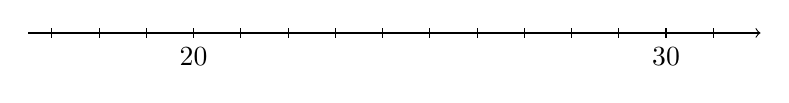
\begin{tikzpicture}[scale=0.6]
  \draw[->] (-0.5,0) -- (15,0);

  \foreach \x in {0,1,2,3,4,5,6,7,8,9,10,11,12,13,14}
    \draw (\x,0.1) -- (\x,-0.1) node[below] {};
  \draw (3,0.1) -- (3,-0.1) node[below] {20};
  \draw (13,0.1) -- (13,-0.1) node[below] {30};

\end{tikzpicture}
\end{center}
\vspace{-0.3cm}

\ligne

\ligne

\end{Exemple}

\begin{Définition}[c]
\textbf{Intercaler} un nombre entre deux autres revient à trouver un nombre compris entre les deux nombres donnés.
\end{Définition}

\begin{Exemple}
\begin{minipage}[c]{.7\textwidth}
Intercaler un nombre entre 21,5 et 21,6 : \ligne

\ligne


\end{minipage} \hfill \begin{minipage}[c]{.3\textwidth}
\begin{center}
\begin{tikzpicture}
  \draw[->] (-0.5,0) -- (2,0);
  \draw (0,0.1) -- (0,-0.1) node[below] {21,50};
  \draw (1.5,0.1) -- (1.5,-0.1) node[below] {21,60};
  \draw[very thick,Couleur8] (0.75,0.2) -- (0.75,-0.2);
\end{tikzpicture}
\end{center}
\end{minipage}

\end{Exemple}

\begin{Définition}[c]
\textbf{Arrondir} un nombre à un rang donné, c'est trouver le nombre le plus proche du nombre initial dont l'écriture s'arrête à ce rang. On utilise le symbole « environ égal : $\simeq$ » entre le nombre et son arrondi.
\end{Définition}

\begin{Exemples}
\begin{itemize}
\item Arrondir à l'unité de 23,7 : \ligne

\item Arrondir au dixième de 91,42 : \ligne

\ligne

\end{itemize}
\end{Exemples}
